\documentclass[class=NCU_thesis, crop=false]{standalone}
\begin{document}

\chapter{研究方法}

\section{資料前處理}
\subsection{擷取HU值範圍}
由於電腦斷層掃描影像原始數值範圍較廣,如\cref{fig:fig-dataset-contrast-range-origin}所示,
數值範圍分布於-3000 HU至3000 HU,然而絕大部分除了-3000 HU(掃描範圍外的背景)以外之數值皆分布在-1000 HU至500 HU的範圍,
若直接使用此影像進行訓練,會因為輸入模型之影像對比度不佳,進而影響後續模型訓練的結果。
\cref{fig:fig-dataset-contrast-origin}為原始影像以灰階圖呈現的結果,可以看出其對於心臟結構以及冠狀動脈之對比度較差。
\fig[0.75][fig:fig-dataset-contrast-range-origin][!hbt]{fig-dataset-contrast-range-origin.jpg}[有顯影劑增強之電腦斷層掃描影像原始數值範圍][有顯影劑增強之電腦斷層掃描影像原始數值範圍]

而在-1000 HU至500 HU的分布範圍中,分布於-1000 HU附近的數值為空氣,分布於-700 HU至-600 HU附近的數值為肺部,
對於冠狀動脈分割較重要的部分如軟組織、顯影劑流經之血管、骨骼之範圍則是分布於-300 HU至500 HU,
因此本研究在資料前處理時,會將原始影像以下界-300 HU以及上界500 HU進行調整,
超過下界數值設為下界,超過上界之數值設為上界,並進行標準化壓縮至-1至1的範圍,
調整後之影像以灰階圖呈現如\cref{fig:fig-dataset-contrast-after-adjustment},可以看出其對於心臟結構以及冠狀動脈之對比度較佳。

\begin{figure}[!hbt]
    %\captionsetup[subfigure]{labelformat=empty} % 完全隱藏圖號
    \centering
    \subcaptionbox
        {調整前
        \label{fig:fig-dataset-contrast-origin}}
        {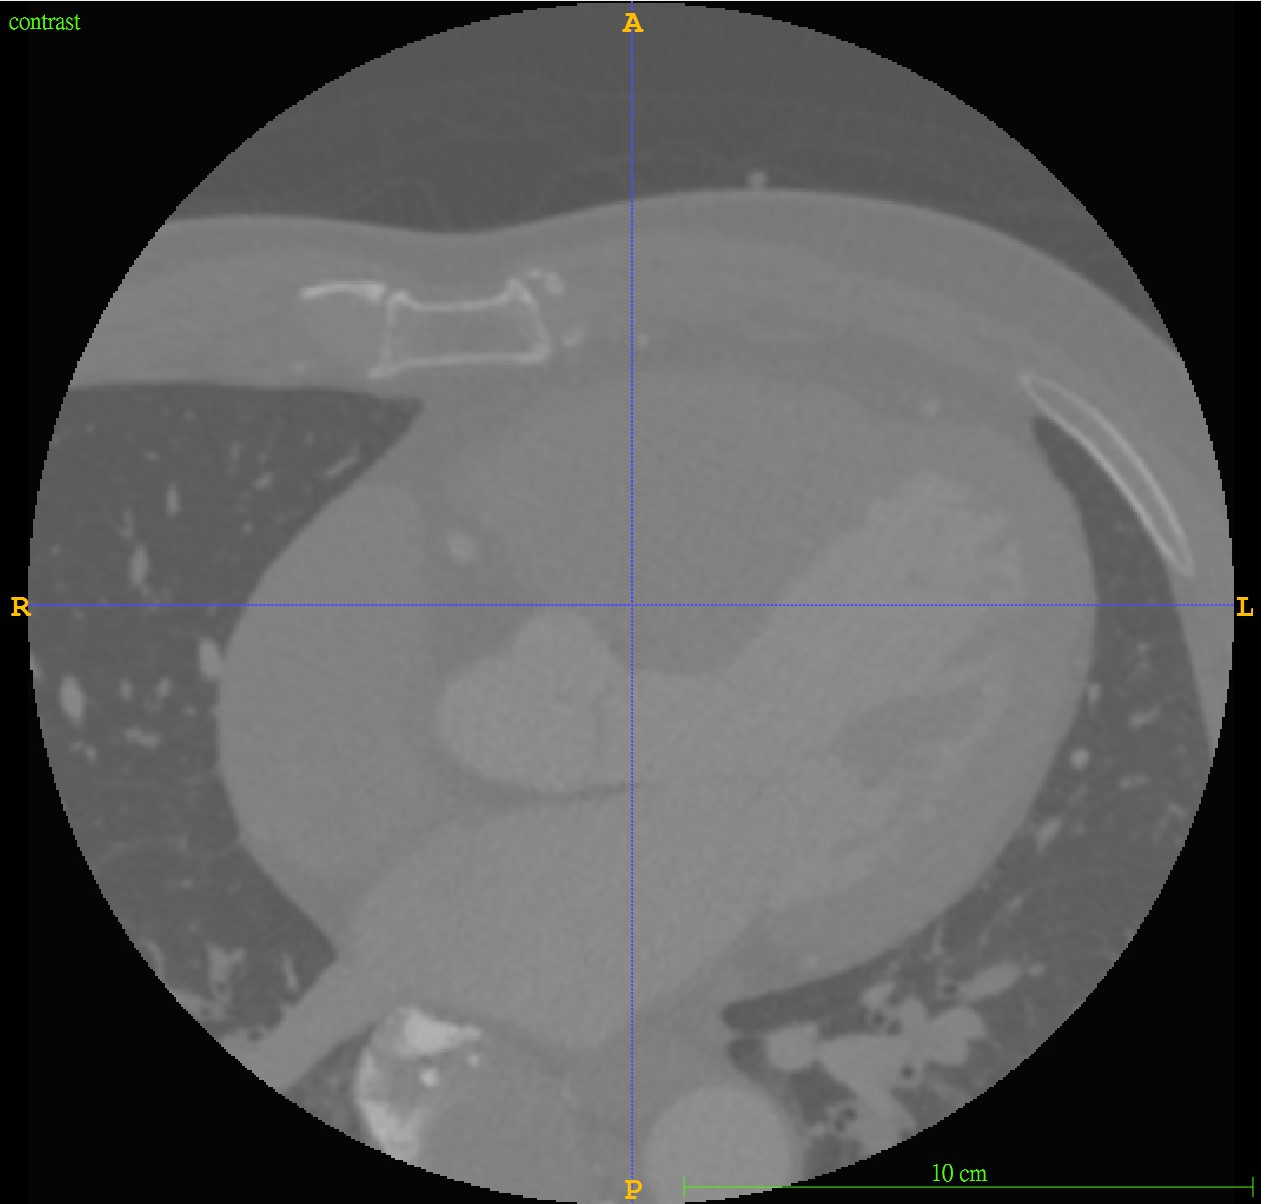
\includegraphics[width=0.4\linewidth]{fig-dataset-contrast-origin}}
    ~
    \subcaptionbox
        {調整後
        \label{fig:fig-dataset-contrast-after-adjustment}}
        {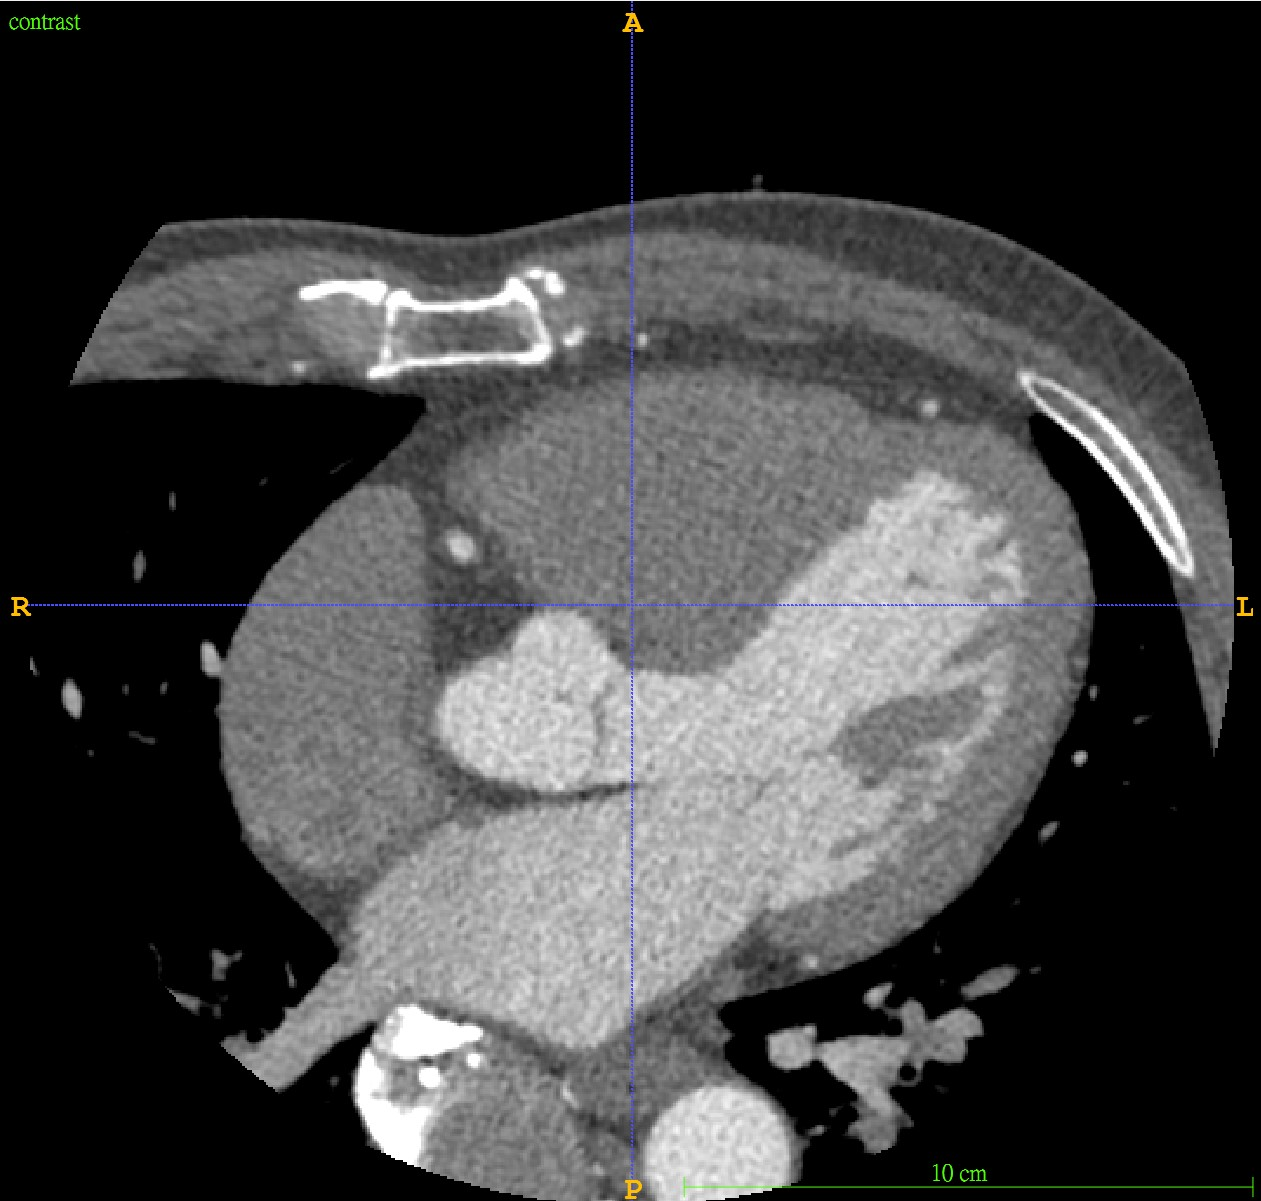
\includegraphics[width=0.4\linewidth]{fig-dataset-contrast-after-adjustment}}
    \caption{有顯影劑增強之電腦斷層影像數值調整}
    \label{fig:fig-dataset-contrast-before-after-adjustment}
\end{figure}

對於無顯影劑增強之電腦斷層影像也依照上述方式,以下界-300 HU以及上界500 HU進行調整。
\cref{fig:fig-dataset-cs-before-after-adjustment}為調整前後之影像以灰階圖呈現的結果。

\begin{figure}[!hbt]
    %\captionsetup[subfigure]{labelformat=empty} % 完全隱藏圖號
    \centering
    \subcaptionbox
        {調整前
        \label{fig:fig-sample-cs-before-adjustment}}
        {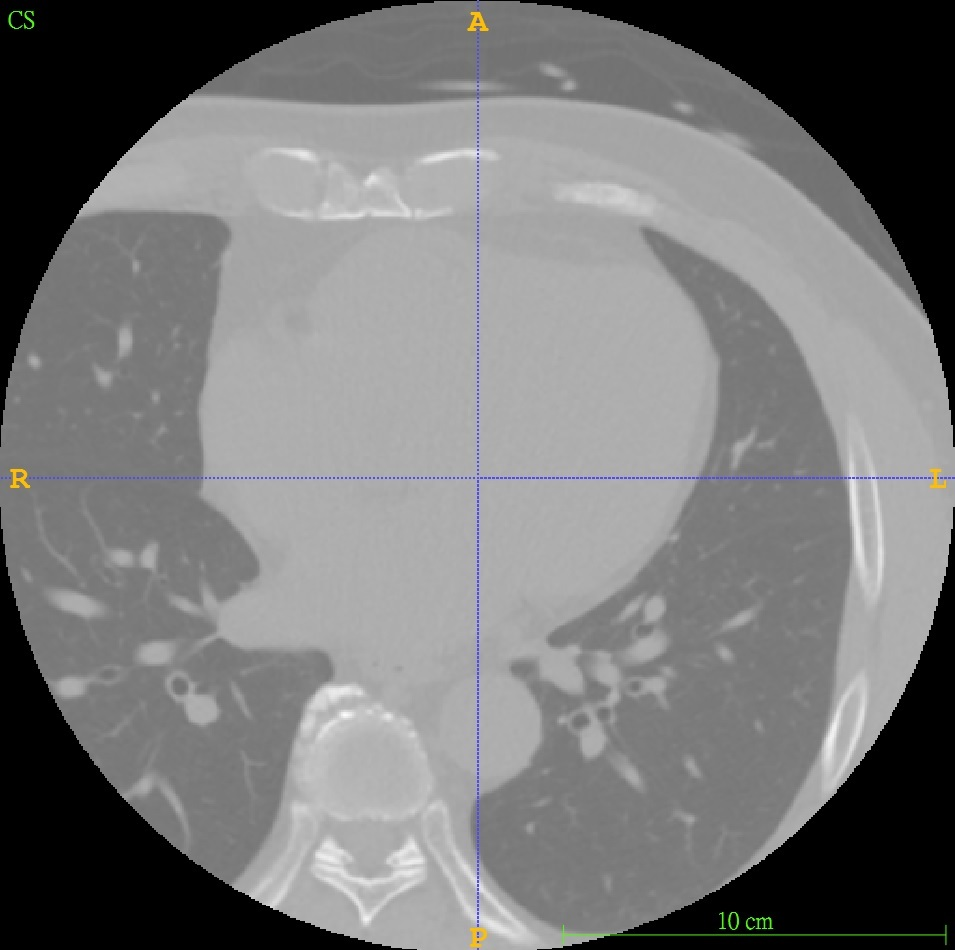
\includegraphics[width=0.4\linewidth]{fig-sample-cs-before-adjustment.jpg}}
    ~
    \subcaptionbox
        {調整後
        \label{fig:fig-sample-cs-after-adjustment}}
        {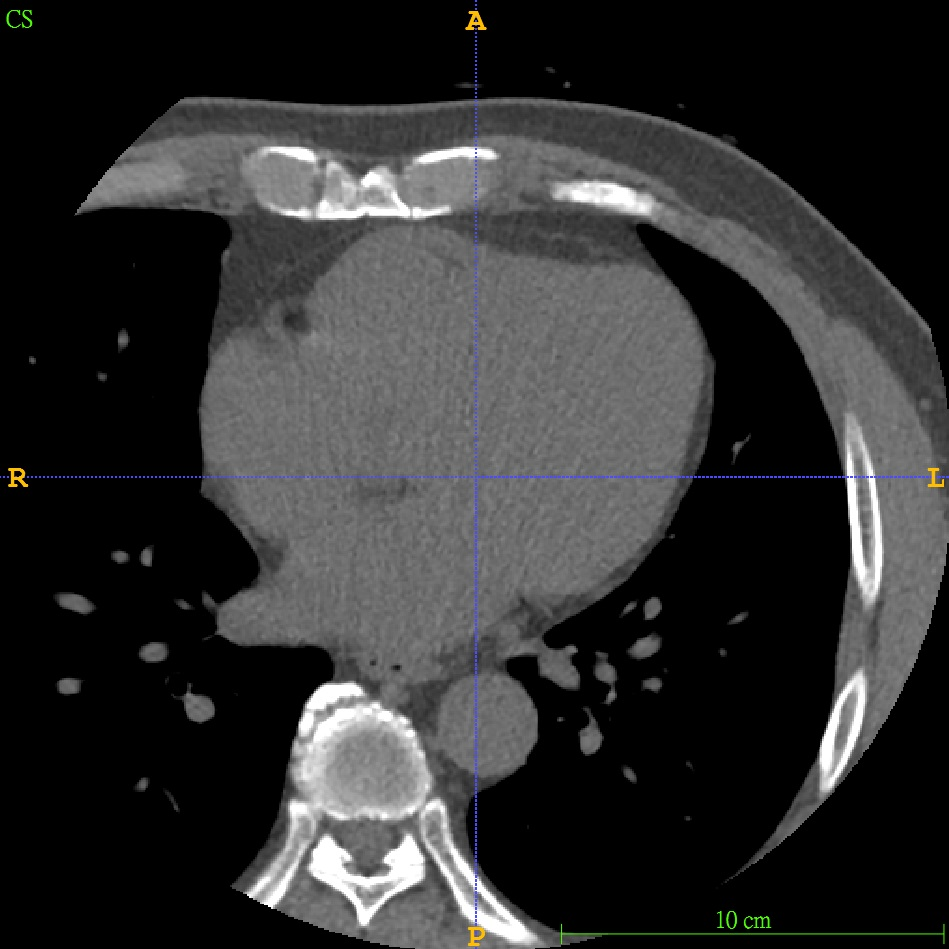
\includegraphics[width=0.4\linewidth]{fig-sample-cs-after-adjustment.jpg}}
    \caption{無顯影劑增強之電腦斷層影像數值調整}
    \label{fig:fig-dataset-cs-before-after-adjustment}
\end{figure}

\subsection{影像壓縮}
由於原始影像大小過於龐大,受限於運算資源,無法一次使用完整的3D影像進行訓練,
因此影像在輸入模型進行訓練、預測前會先進行圖片大小壓縮,
並將模型輸出結果以線性內插轉換回原始大小進行評估。
\cref{table:table-image-size-compress}為原始影像大小以及壓縮後的大小,
\cref{table:table-image-size-compress}中的數值分別為三維影像之長、寬、高像素數量。
\begin{table}[h]
    \centering
    \caption{原始影像大小及壓縮後大小}
    \label{table:table-image-size-compress}
    \begin{tabular}{|c|c|c|}
    \hline
    名稱 & 原始影像大小 & 壓縮後大小 \\
    \hline
    有顯影劑增強影像 & (512, 512, 256) & (192, 192, 192) \\
    \hline
    無顯影劑增強影像 & (512, 512, 64) & (256, 256, 64) \\
    \hline
    \end{tabular}
\end{table}

\section{無顯影劑影像資料擴增模型}
\cref{fig:fig-sample-with-without-contrast}為自同一受檢者拍攝之有、無顯影劑之電腦斷層影像,
從資料中可以觀察到無顯影劑增強之電腦斷層影像對於血管對比度較低,在有顯影劑增強之電腦斷層影像,如\cref{fig:fig-sample-contrast}中,心臟血液流經的部分為白色,與其他組織較有差異性;
而在無顯影劑增強之電腦斷層影像,如\cref{fig:fig-sample-cs}中,心臟血液流經的部分則與其他組織較無差異。
\begin{figure}[!hbt]
    %\captionsetup[subfigure]{labelformat=empty} % 完全隱藏圖號
    \centering
    \subcaptionbox
        {有注射顯影劑
        \label{fig:fig-sample-contrast}}
        {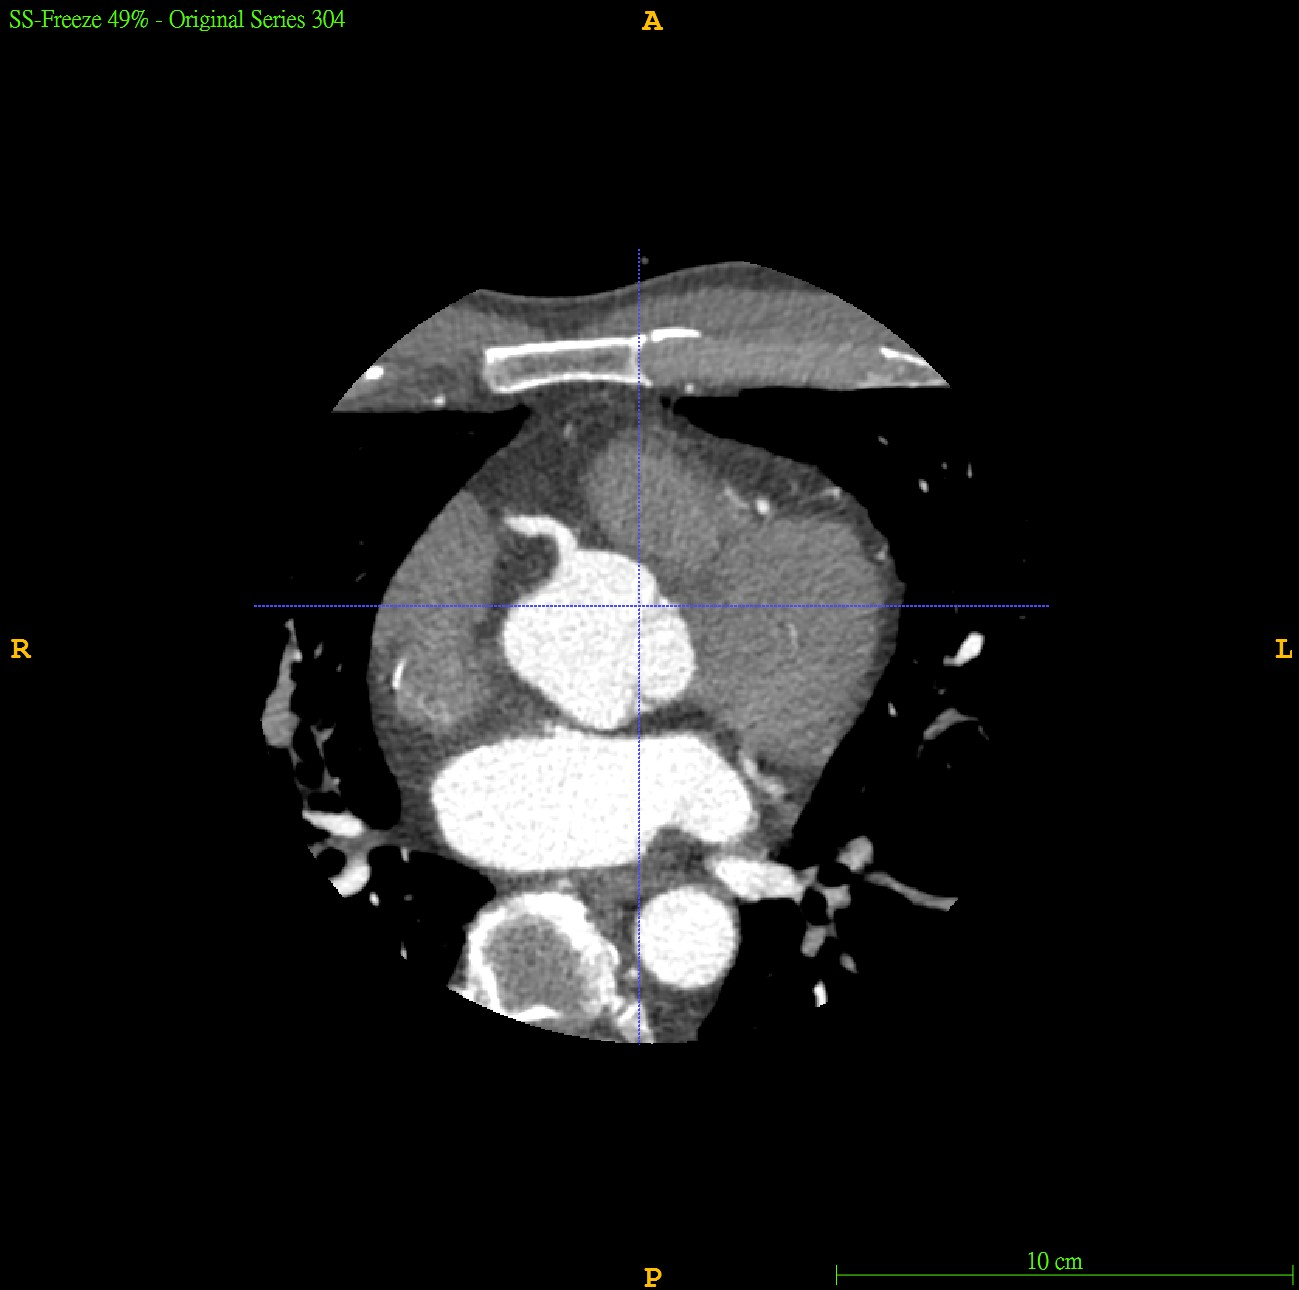
\includegraphics[width=0.475\linewidth]{fig-sample-contrast.jpg}}
    ~
    \subcaptionbox
        {無注射顯影劑
        \label{fig:fig-sample-cs}}
        {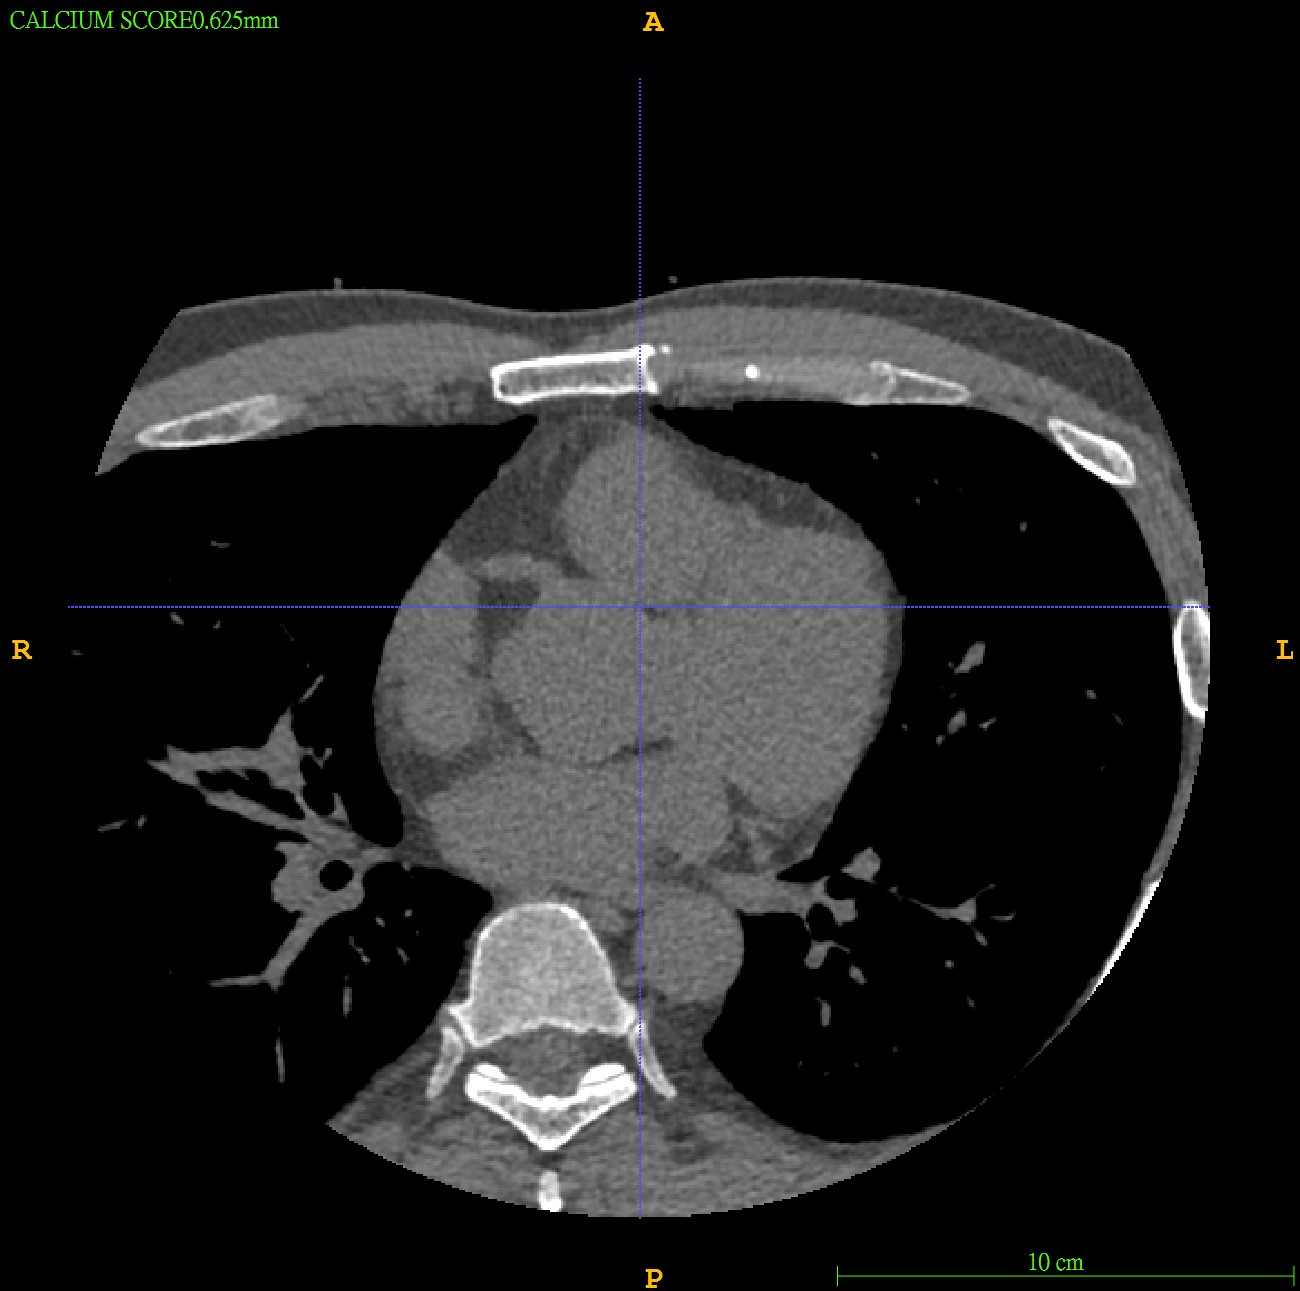
\includegraphics[width=0.475\linewidth]{fig-sample-cs.jpg}}
    \caption{有無顯影劑增強之電腦斷層影像}
    \label{fig:fig-sample-with-without-contrast}
\end{figure}

此種差異增加了標記資料的難度,使得原本就需要耗費大量時間的人工標記血管任務,
在無顯影劑增強的電腦斷層影像中更為困難,
且標記之血管結果不如血管對比度較高的有顯影劑增強之電腦斷層影像,
使得取得品質優良之標記資料難度也更高。

一個能利用既有資料輔助訓練的想法是,
將已標記之有顯影劑增強之電腦斷層掃描影像進行影像風格轉換,
將其轉換為無顯影劑增強之電腦斷層掃描影像做為額外的訓練資料。
其中CycleGAN已被許多研究用於醫學影像之影像風格轉換研究
~\cite{jiangTumorAwareAdversarialDomain2018, welanderGenerativeAdversarialNetworks2018, songNoncontrastCTLiver2020},
目前也有研究使用深度學習技術進行醫學影像的轉換,並用於資料擴增的任務上~\cite{songNoncontrastCTLiver2020}。

本研究使用CycleGAN訓練一個影像風格轉換模型,
將有顯影劑增強之電腦斷層影像轉換為虛擬的無顯影劑增強之電腦斷層影像,
即是將\cref{fig:fig-sample-contrast}轉換為\cref{fig:fig-sample-cs},
並使用在有顯影劑增強之電腦斷層影像標註之冠狀動脈分割標記,
做為無顯影劑增強之電腦斷層影像冠狀動脈分割任務的擴充資料,
期望能以現有資料增加分割模型的效果。

有無使用CycleGAN對於訓練無顯影劑增強之電腦斷層影像冠狀動脈分割模型的結果,
會在實驗設計與結果的章節進行討論。

\section{冠狀動脈分割}
目前已有許多研究
~\cite{huangCoronaryArterySegmentation2018, chenCoronaryArterySegmentation2019}
對於有顯影劑增強之電腦斷層影像進行冠狀動脈分割的任務達成不錯的成果,
3D U-Net是其中被廣泛運用於醫學影像分割的模型,因此本研究使用3D U-Net做為冠狀動脈分割任務之模型。

模型訓練所使用的目標函數為骰子損失函數(Dice Loss),其函式為\cref{eqn:dice-loss}
\begin{equation}
\label{eqn:dice-loss}
Loss = 1-\frac{2|X\cap Y|}{|X|+|Y|} 
\end{equation}
其中X、Y分別為模型預測結果以及模型預期結果,
當兩者重疊部分越多且不重疊部分越少時,損失數值越低,反之則愈高。

雖然有顯影劑增強之電腦斷層影像相較於無顯影劑增強之電腦斷層影像能夠更精確地顯示血管位置,
並取得較佳的冠狀動脈分割結果,然而部分對於碘成分過敏或是腎臟功能有問題的受檢者,
可能會對顯影劑產生不良反應
~\cite{andreucciUpdateRenalToxicity2017,rasuliMetforminContrastMedia1998,saljoughianIntravenousRadiocontrastMedia2012},
這些受檢者較不適合使用顯影劑,
因此本研究也實驗了以無顯影劑增強之電腦斷層影像進行冠狀動脈分割實驗,
期望提供不適合注射顯影劑的受檢者初步的冠狀動脈分割,
以輔助醫師在後續的診斷流程。


\section{有顯影劑冠狀動脈分割之相關應用}
\subsection{鈣化位置偵測}
目前在進行完整的冠狀動脈疾病風險評估時,
會需要同時使用有顯影劑以及無顯影劑增強之影像,
分別進行冠狀動脈分割以及鈣化位置偵測,
流程如\cref{fig:fig-contrast-cs-ct-examination}所示,
在進行電腦斷層掃描攝影時,
受檢者會先在無注射顯影劑時進行電腦斷層影像攝影,
取得無顯影劑增強之電腦斷層影像,接著再接受顯影劑注射,
進行第二次電腦斷層影像攝影取得有顯影劑增強之電腦斷層影像。

\fig[0.2][fig:fig-contrast-cs-ct-examination][!hbt]{fig-contrast-cs-ct-examination.jpg}[冠狀動脈疾病風險評估流程][冠狀動脈疾病風險評估流程]

有顯影劑增強之影像將會利用於標註冠狀動脈結構,
使得醫師能夠了解受檢者的冠狀動脈結構、是否有血管狹窄度的情形,
無顯影劑增強之影像則會利用於鈣化位置標註,
使得醫師能夠了解受檢者的冠狀動脈是否有鈣化以及鈣化的位置,
將冠狀動脈結構以及鈣化位置搭配進行參考,
能夠更精確地了解鈣化在血管中的位置。

然而在這樣的流程下,受檢者會需要接受兩次的電腦斷層影像攝影,
接受兩次的輻射暴露,
因此本研究希望能直接使用有顯影劑增強之電腦斷層影像進行鈣化位置評估,
透過提供醫生輸入欲擷取之HU值閥值,
利用血管分割模型的結果擷取出血管周遭的鈣化位置並以視覺化呈現,
使得受檢者只需進行一次有注射顯影劑之電腦斷層掃描攝影,
便能找到其血管中可能有鈣化的位置,
降低受到輻射暴露的風險。

\fig[0.2][fig:fig-contrast-calcium-location][!hbt]{fig-contrast-calcium-location.jpg}[僅以有顯影劑資料進行鈣化位置偵測流程][僅以有顯影劑資料進行鈣化位置偵測流程]

本研究的流程如\cref{fig:fig-contrast-calcium-location}所示,
受檢者會在注射顯影劑後進行電腦斷層掃描攝影,
透過本研究提出之冠狀動脈分割模型進行自動冠狀動脈分割,
並使用冠狀動脈分割結果、原始電腦斷層影像、以及使用者輸入之目標HU閥值,
透過取三者之交集,將血管位置中超過使用者輸入HU閥值之位置視為鈣化位置,
並將其以視覺化呈現,提供醫生進行診斷時參考。


\subsection{狹窄度分析}
在冠狀動脈心臟病的診斷中,血管狹窄度是一個重要的指標,
目前醫師可以透過電腦斷層掃描影像或分割之血管結果,
了解受檢者之血管管徑趨勢,藉以診斷受檢者是否有血管狹窄的情形。

然而單純以目視的方式難以精準的了解受檢者之血管管徑數據,
且冠狀動脈是一個在三維空間中往不同方向發展的結構,
在判斷血管管徑時會需要考慮到不同觀察方向,
也使得進行診斷時的不便,
因此本研究期望能提供醫師於血管狹窄度分析時更方便的資料,
藉由冠狀動脈分割結果取得其中心線,
將原始影像轉換為以中心線投影之拉直後之影像,
使得更容易的看出血管管徑趨勢,
此外,本研究也以拉直後之影像計算血管管徑並繪製成趨勢圖,
以方便醫師進行對血管狹窄度的分析。

\fig[0.25][fig:fig-stenosis-detection][!hbt]{fig-stenosis-detection.jpg}[狹窄度分析流程][狹窄度分析流程]

\begin{figure}[!hbt]
    %\captionsetup[subfigure]{labelformat=empty} % 完全隱藏圖號
    \centering
    \subcaptionbox
        {原始分割結果
        \label{fig:fig-before-skeleton}}
        {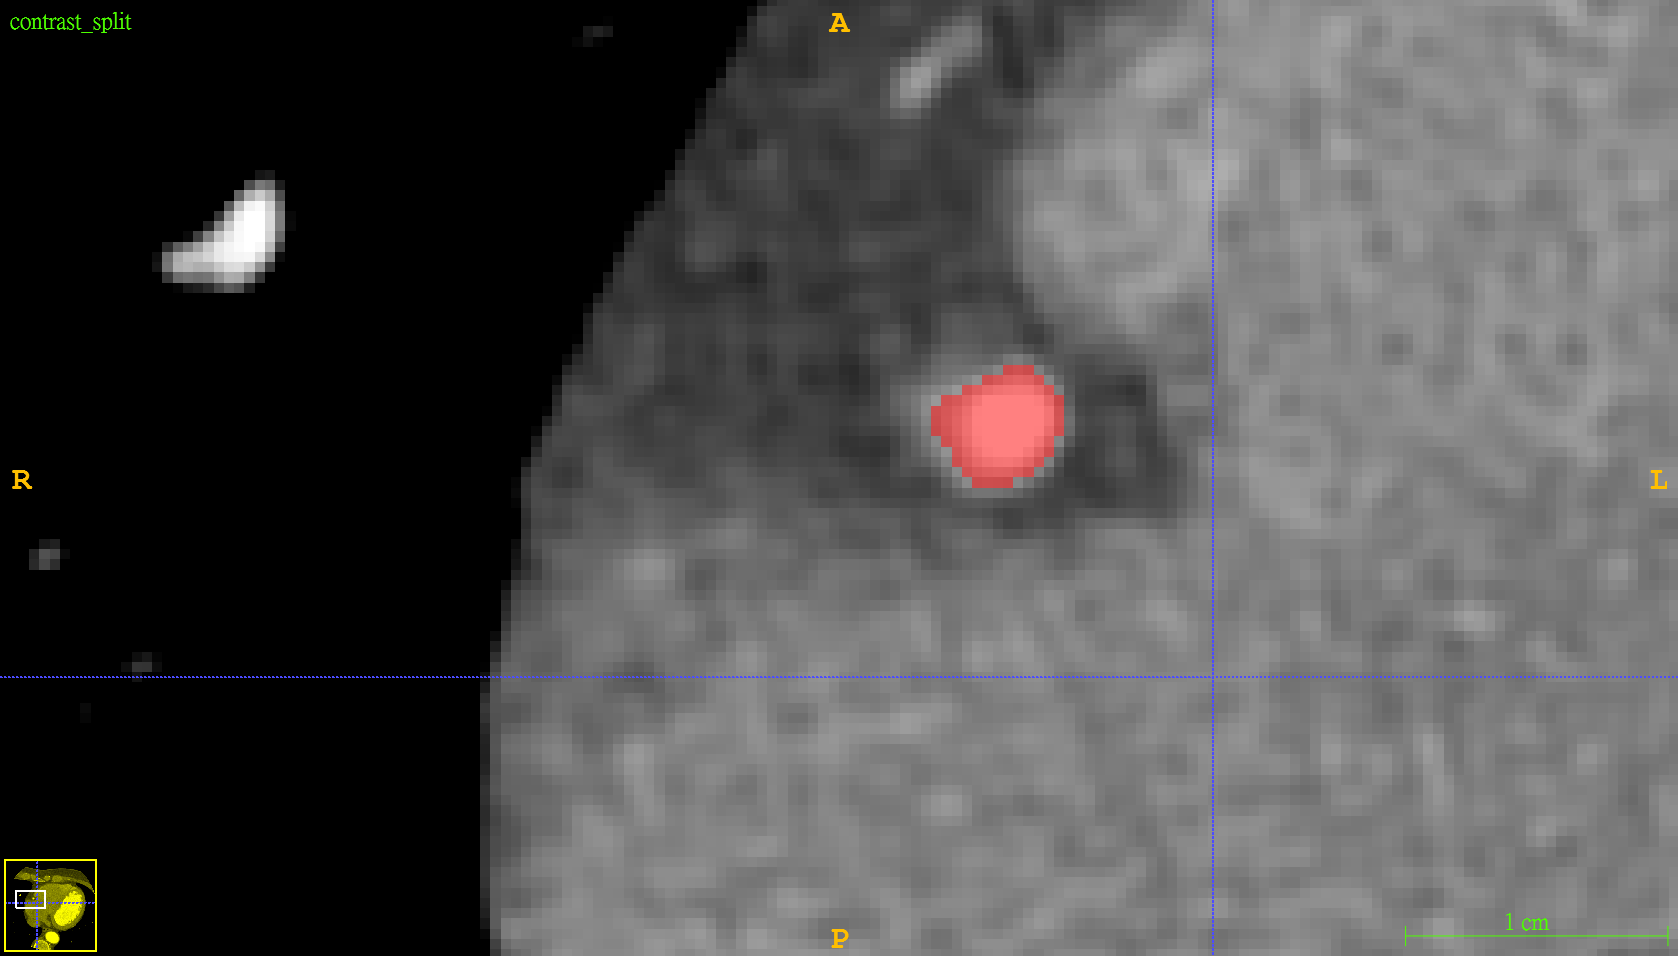
\includegraphics[width=0.475\linewidth]{fig-before-skeleton.jpg}}
    ~
    \subcaptionbox
        {細線化之結果
        \label{fig:fig-after-skeleton}}
        {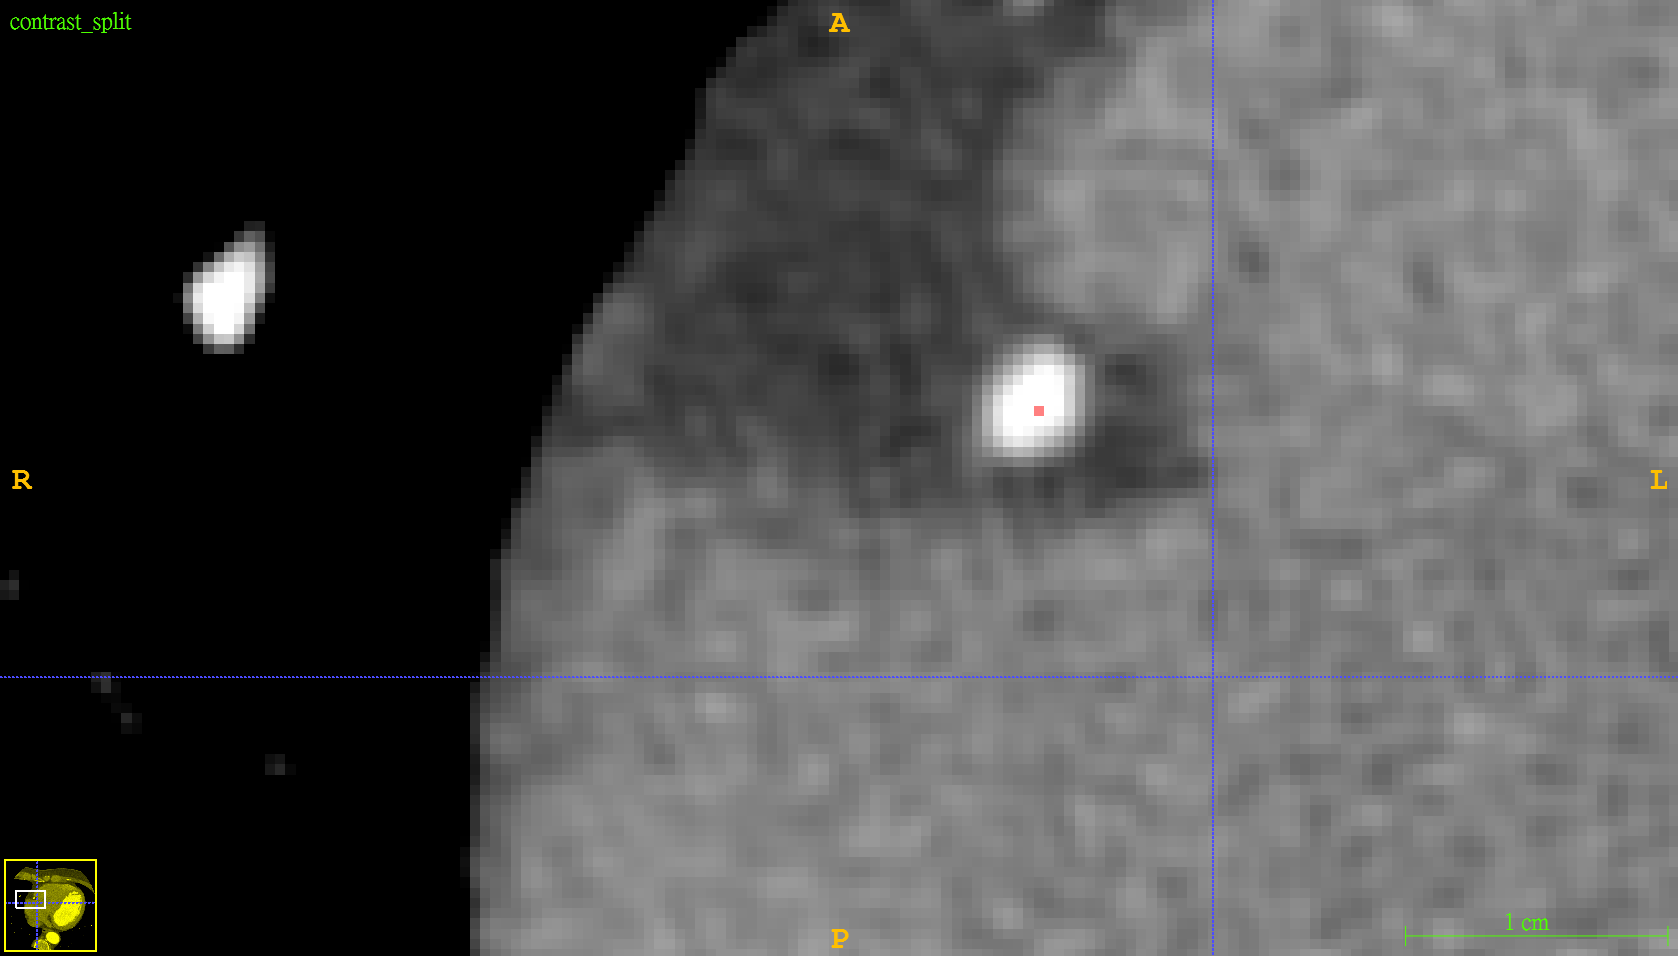
\includegraphics[width=0.475\linewidth]{fig-after-skeleton.jpg}}
    \caption{細線化處理取得中心線}
    \label{fig:fig-skeleton}
\end{figure}

\fig[0.75][fig:fig-cpr-y][!hbt]{fig-cpr-y.jpg}[以血管中心線拉直之原始影像][以血管中心線拉直之原始影像]

\begin{figure}[!hbt]
    %\captionsetup[subfigure]{labelformat=empty} % 完全隱藏圖號
    \centering
    \subcaptionbox
        {原始分割結果
        \label{fig:fig-before-cpr}}
        {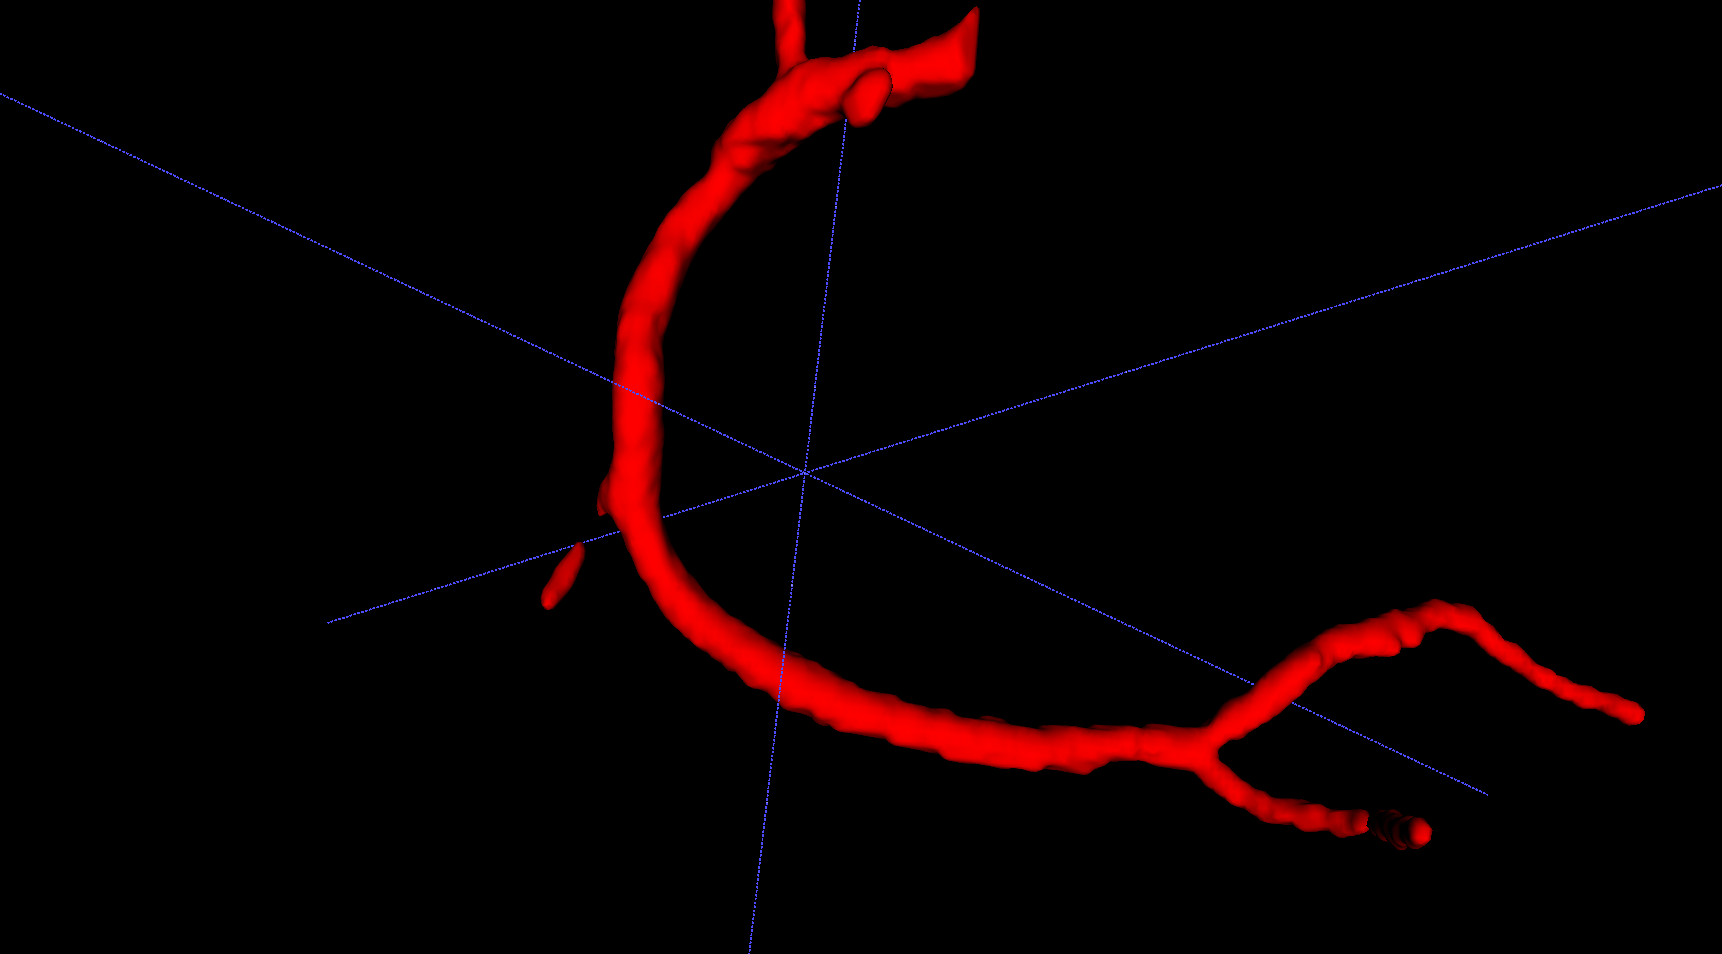
\includegraphics[width=0.475\linewidth]{fig-before-cpr.jpg}}
    ~
    \subcaptionbox
        {利用中心線拉直之結果
        \label{fig:fig-after-cpr}}
        {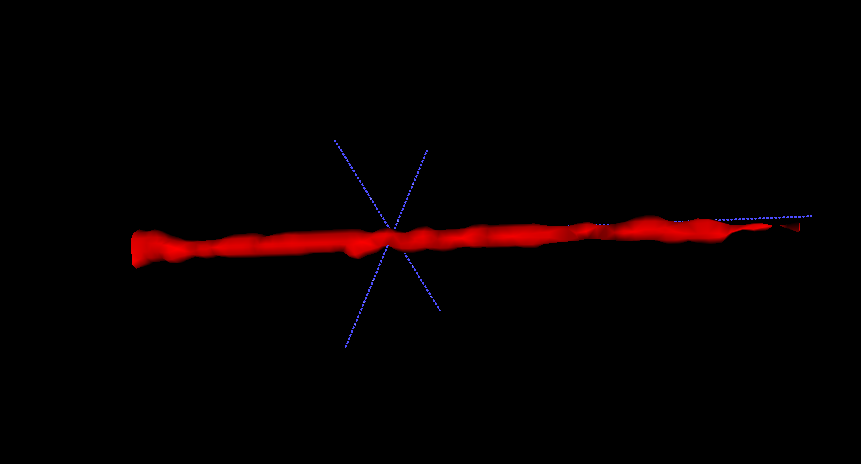
\includegraphics[width=0.475\linewidth]{fig-after-cpr.jpg}}
    \caption{以血管中心線拉直之冠狀動脈分割}
    \label{fig:fig-cpr}
\end{figure}

本研究之狹窄度分析流程如\cref{fig:fig-stenosis-detection}所示,
首先會透過原始影像中分割出冠狀動脈結構,
並將分割結果進行細線化處理取得中心線,
中心線轉換的結果如\cref{fig:fig-skeleton},
\cref{fig:fig-skeleton}中紅色部分分別為原始分割結果以及細線化得到之中心線,
接著利用Curved Planar Reformation方法~\cite{kanitsarCPRCurvedPlanar2002}以血管中心線對原始影像進行座標轉換,
為利用血管中心線做為向量,產生以中心線之拉直後之影像,
原始影像以RCA主支中心線進行轉換的結果如\cref{fig:fig-cpr-y},
\cref{fig:fig-cpr-y}之結果會用提供給使用者做為額外的參考資料,
\cref{fig:fig-cpr}冠狀動脈分割以RCA主支中心線進行轉換的結果,
本研究會利用轉換後之冠狀動脈分割計算血管管徑,
並繪製成趨勢圖,以方便醫師進行對血管狹窄度的分析。


\subsection{資料視覺化}
本研究使用開源軟體3D Slicer
~\cite{theslicercommunity3DSlicerImage,fedorov3DSlicerImage2012,geringIntegratedVisualizationSystem1999,geringIntegratedVisualizationSystem2001,kapurIncreasingImpactMedical2016,kikinis3DSlicerPlatform2014,pieperNAMICKitITK2006}
做為資料視覺化平台,軟體介面如\cref{fig:fig-3dslicer-ul-example}。
\fig[0.75][fig:fig-3dslicer-ul-example][!hbt]{fig-3dslicer-ul-example.jpg}[3D Slicer軟體介面][3D Slicer軟體介面]

\fig[0.5][fig:fig-3dslicer-custom-extension-example][!hbt]{fig-3dslicer-custom-extension-example.jpg}[3D Slicer自定義套件][3D Slicer自定義套件]

3D Slicer提供多平台的桌面應用程式,
能在Windows, Linux, MacOS上運行,
並且支援多種格式的醫學影像資料、資料檢視方式以及資料處理工具,
此外,使用者能夠利用Python撰寫自定義的3D Slicer套件,
使得使用者能在3D Slicer中呼叫自行撰寫的Python程式、深度學習模型進行資料處理,
並將結果回傳至3D Slicer進行呈現。

本研究將冠狀動脈分割模型、鈣化位置分析模組、狹窄度分析模組以3D Slicer套件的形式整合至3D Slicer中,
套件介面如\cref{fig:fig-3dslicer-custom-extension-example},
使用者可以將心臟電腦斷層影像匯入至3D Slicer,
選取來源影像、是否有顯影劑以及HU範圍呼叫深度學習模型進行冠狀動脈自動標記。
對於有顯影劑影像所擷取出之冠狀動脈,可以設定HU閥值呼叫鈣化位置分析模組進行鈣化位置偵測,
此外,使用者能夠選取血管的兩端點呼叫狹窄度分析模組,
取得以中心線拉直後血管影像以及血管管徑趨勢圖。

\end{document}